\documentclass[../piano-di-progetto.tex]{subfiles}
\begin{document}
\subsection{consolidamento dei requisiti}
Il periodo di consolidamento dei requisiti inizia il 2020-04-14 e termina il giorno 2020-04-20, prima della revisione dei requisiti. 

\subsubsection{Ruoli}
Durante questa macro, viene richiesta la presenza dei seguenti ruoli:
\begin{itemize}
    \item Responsabile;
    \item Amministratore;
    \item Analista;
    \item Verificatore.
\end{itemize}

\subsubsection{Attività}
Durante questo macro periodo verranno svolte le seguenti attività:
\begin{itemize}
    \item \textbf{Preparazione della presentazione}: viene creata la presentazione che verrà esposta durante la revisione di avanzamento;
    \item \textbf{Analisi dei requisiti}: revisione dei requisiti;
    \item \textbf{Verifica}.
\end{itemize}


\newpage
\begin{landscape}
    \begin{figure}[H]
        \centering
        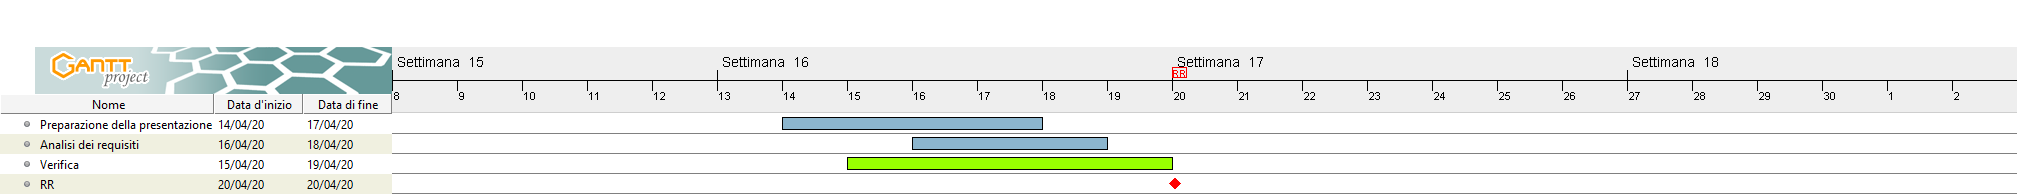
\includegraphics[width=24cm]{img/consolidamento.png}
        \caption{Diagramma attività nel periodo di consolidamento dei requisiti}
      \end{figure}
\end{landscape}

\end{document}